\documentclass[12pt,a4paper]{article}

\usepackage[utf8]{inputenc}
\usepackage[T1]{fontenc}
\usepackage[left=2.5cm,right=2.5cm,top=2.5cm,bottom=2.5cm]{geometry}
\usepackage{graphicx}
\usepackage{longtable}
\usepackage{array}
\usepackage{tabularx}
\usepackage{hyperref}
\usepackage{xcolor}
\usepackage{booktabs}
\usepackage{enumitem}
\usepackage{amsmath}
\usepackage{natbib}

\hypersetup{
    colorlinks=true,
    linkcolor=blue!70!black,
    urlcolor=blue!60!black,
    citecolor=green!50!black,
}

\title{Software Design Document\\[2pt]
\large AI-Assisted Discovery of Dynamic Graph Algorithms\\ via Evolutionary Code Repair}
\author{Thonmay Md Thoriqul Islam\\
\textit{E\"otv\"os Lor\'and University, Faculty of Informatics}\\
\small Supervisor: Gregory Reynolds Morse}
\date{September 2026}

\begin{document}
\maketitle

% ============================================================
% Version / revision history
% ============================================================
\begin{center}
\renewcommand{\arraystretch}{1.25}
\begin{tabular}{|c|c|p{8.5cm}|}
\hline
\textbf{Version} & \textbf{Date} & \textbf{Revision note} \\
\hline
v0.1 & Jul 2026 & Initial design draft (pre-audit). \\
\hline
v0.2 & Sep 2026 & Revised after checkpoint-3 audit: corrected DFS/LBFS invariants, real OS-level sandbox, interactive dashboard UI restored, atomic JSON persistence, single candidate state machine, twelve-class model, contribution traceability, bounded-verification claims, three provisional final-exam topics, and Thesis Consultation registration note. \\
\hline
\end{tabular}
\end{center}

\tableofcontents
\clearpage

% ============================================================
\section{System Overview}
\label{sec:overview}

\subsection{Purpose}

This document is the software design for a research platform that discovers correct and efficient \emph{dynamic} graph algorithms through LLM-driven evolutionary code repair. A dynamic algorithm maintains a structural property (a BFS tree, a DFS forest, a strongly connected component decomposition, an MCS ordering, or a LexBFS ordering) incrementally under edge insertions and deletions, instead of recomputing it from scratch after every update. The platform combines AI-based code generation and repair with an exhaustive, isomorphism-aware, trusted verification engine, and wraps both in an evolutionary search loop.

The document's goal is to be implementable: a reader who has not seen the code should be able to build the principal modules, the data model, the interaction surfaces, and the verification pipeline from this design alone, without inventing the core decisions.

\subsection{Scope and Problem Tiers}

The platform operates on a fixed graph representation, an \textbf{adjacency matrix of zeros and one}, and supports a tiered set of target problems. The tiers are locked and are not a research question:

\begin{itemize}[noitemsep]
  \item \textbf{Calibration (directed):} dynamic BFS and dynamic DFS. Known correct solutions exist and are used to validate the verifier before any experiment.
  \item \textbf{Primary target (undirected):} dynamic MCS (Maximum Cardinality Search). MCS produces perfect elimination orderings for chordal graphs \cite{tarjan1984mcs,heggernes2006} and is the main discovery target.
  \item \textbf{Harder / open (directed):} dynamic SCC and dynamic Lexicographic BFS (LBFS).
\end{itemize}

Reachability is in scope as a secondary directed problem and is given an invariant in Section~\ref{sec:invariants}. The system runs experiments autonomously and reports both positive results (a discovered correct algorithm) and negative results (where and why the search fails). Both are valid scientific outcomes.

\subsection{Key Concepts}

\begin{description}[style=nextline, leftmargin=2cm]
  \item[Candidate] One attempt at a dynamic algorithm, stored as executable Python code implementing a fixed update interface.
  \item[Generation] One round of generate, test, reflect, select.
  \item[Population] The set of candidates alive at one time; typically 5--20 candidates.
  \item[Fitness] A score measuring candidate quality: the fraction of test sequences on which the invariant holds after every operation.
  \item[Invariant] A property that must always hold for a correct algorithm. Correctness is judged by the invariant, not by equality to a reference output, because dynamic outputs are generally non-unique.
  \item[Reflection] LLM analysis of why a candidate failed, structured and reused to guide repair.
  \item[Work ratio] $\text{work\_ratio} = \text{candidate\_work} / \text{offline\_recomputation\_work}$; an efficiency improvement requires $\text{work\_ratio} < 1$.
  \item[Trusted verifier] Pre-built, validated infrastructure that tests candidates. No agent can read or modify it.
\end{description}

\subsection{Four Distinct Correctness Claims}

A recurring audit defect was the conflation of ``exhaustive testing'' with ``proof''. This design separates four claims, and every statement in the document is labelled with the claim it makes:

\begin{enumerate}[noitemsep]
  \item \textbf{Tool correctness.} The research tool itself (orchestrator, verifier, persistence) is correct. This is established by unit tests and by validating the verifier against known-good and known-bad inputs.
  \item \textbf{Bounded candidate verification.} A discovered candidate has \emph{no counterexample within the stated bound} (all non-isomorphic digraphs up to $n \le 5$, and operation sequences up to a stated length). This is \emph{not} a proof of correctness for arbitrary size or update length.
  \item \textbf{Search effectiveness.} The evolutionary loop finds a correct candidate within a stated generation budget. This is an empirical, statistical claim over repeated runs.
  \item \textbf{Mathematical proof.} A formal proof that a discovered algorithm is correct for all inputs. This is reserved for the final Lean~4 phase (Section~\ref{sec:lean}) and is explicitly \emph{not} claimed by the verification engine.
\end{enumerate}

The verification engine delivers claim (2). The Lean phase targets claim (4). Conflating them is forbidden: any sentence asserting a candidate is ``correct'' must state its bound.

% ============================================================
\section{Related Work and Complexity Bounds}
\label{sec:related}

This section places the discovery target, dynamic Maximum Cardinality Search (MCS), in the context of two bodies of prior work: the static MCS and chordality literature, and the dynamic chordality-maintenance literature. It also states the complexity bounds that frame the realistic research goal. Every citation is to a work whose bounds were verified against the primary source; cells in the summary table that could not be verified are marked \textit{open} or \textit{n/a} rather than given a number.

\subsection{Static MCS and Chordality}

MCS is the linear-time procedure of Tarjan and Yannakakis for testing chordality and for constructing a perfect elimination ordering (PEO) of a chordal graph \cite{tarjan1984mcs}. A static run of MCS reads the entire graph and produces the ordering in $\Theta(n+m)$ time, which is input-optimal: any algorithm that inspects the graph must at least read it. For chordal inputs the resulting ordering is a PEO, and the classic $O(n+m)$ PEO check (the later neighbors of each vertex form a clique) certifies it \cite{tarjan1984mcs,heggernes2006}.

It is worth separating two related but distinct static results. Rose, Tarjan, and Lueker's vertex-elimination work \cite{rose1976algorithmic} is an earlier, different paper: it studies lexicographic search and vertex elimination and is the ancestor of lexicographic BFS (LBFS). It is not the MCS paper, and the two are not conflated here. MCS \cite{tarjan1984mcs} and the elimination/LBFS line \cite{rose1976algorithmic} are separate contributions that happen to both produce orderings useful for chordality.

\subsection{Dynamic Chordality Maintenance: The Promise Model}

The dynamic chordality literature maintains a certificate of chordality under edge insertions and deletions. A defining feature of this line of work is that it operates under a \emph{promise}: before an edge flip is applied, the structure first \emph{queries} whether the flip preserves chordality, and it updates only when the answer is yes. None of the verified works in this line handles a flip that \emph{breaks} chordality.

\begin{itemize}[noitemsep]
  \item \textbf{Ibarra} \cite{ibarra2008dynamic} maintains a clique tree of a chordal graph. The structure queries whether an edge insertion or deletion preserves chordality and updates only when it does.
  \item \textbf{Banerjee, Raman, and Satti} \cite{banerjee2018maintaining} improve the upper and lower bounds. The structure maintains a PEO, detects chordality in $O(\min\{\deg(u),\deg(v)\})$, and updates in $O(\deg(u)+\deg(v))$ when chordality is preserved. The same paper proves an $\Omega(\log n)$ amortized cell-probe lower bound (word size $\log n$) for \emph{any} dynamic structure that maintains a chordal graph.
  \item \textbf{Mezzini} \cite{mezzini2012fully} gives an $O(1)$ query-time and $O(n^2)$ update-time algorithm, again in the promise model.
  \item \textbf{Berry, Sigayret, and Spinrad} \cite{berry2005faster} give faster dynamic chordality maintenance, also in the promise model.
\end{itemize}

\subsection{The Novelty Gap}

The thesis problem is defined on \emph{arbitrary} graphs, not on chordal ones. MCS produces a vertex ordering whether or not the graph is chordal, and the discovery target is to maintain that ordering under edge flips with no chordality promise. This is a different problem from the one the dynamic chordality literature addresses, because that literature assumes the promise that each applied flip preserves chordality and therefore never has to update through a flip that breaks it.

The gap is two independent layers, each of which is claimable on its own:

\begin{enumerate}[noitemsep]
  \item \textbf{Deterministic MCS ordering.} Maintaining the \emph{specific} MCS ordering with a fixed tie-break (the lowest vertex id chosen on ties) under edge updates. Across a thorough literature search, no published sub-$O(n+m)$ per-update algorithm was found for this deterministic variant.
  \item \textbf{MCS-style ordering without the promise.} Maintaining any MCS-style ordering under flips that are \emph{not} promised to preserve chordality. This is open because the entire dynamic chordality literature assumes the promise.
\end{enumerate}

The second layer is the stronger headline, because it does not depend on the tie-break subtlety of the first: even setting aside which MCS ordering is maintained, the literature does not address updates that break chordality.

\subsection{Lower-Bound Caveat}

A tempting claim is that the thesis problem ``inherits'' the $\Omega(\log n)$ lower bound of \cite{banerjee2018maintaining} for free. That claim is \emph{not} established, and this design does not make it. The Banerjee et al.\ bound is proven for maintaining a chordal graph \emph{including} a chordality-detection query. Maintaining the MCS ordering does not give that query for free: deciding whether a stored ordering is a PEO costs $O(n+m)$, so the ordering alone does not answer the chordality query that the lower bound is parameterized on. At most, a weakened version of the bound restricted to the chordal-promise subcase survives, and even that is not proven. The question of whether any $\Omega(\log n)$-type lower bound applies to maintaining the MCS ordering on arbitrary graphs is therefore left as an open question, not stated as a result.

\subsection{Bounds Summary}

Table~\ref{tab:bounds} summarizes the verified bounds. The rows for the dynamic chordality line are stated in the promise model; the thesis row is the target and is marked \textit{open}.

\begin{longtable}{|>{\raggedright\arraybackslash}p{3.6cm}|>{\centering\arraybackslash}p{1.7cm}|>{\centering\arraybackslash}p{1.7cm}|>{\centering\arraybackslash}p{1.6cm}|>{\centering\arraybackslash}p{2.1cm}|>{\raggedright\arraybackslash}p{2.6cm}|}
\caption{Complexity bounds for static MCS, dynamic chordality maintenance, and the thesis target. ``Promise model'' rows assume each applied flip preserves chordality. Unverified cells are marked \textit{open} or \textit{n/a}.}
\label{tab:bounds} \\
\hline
\textbf{Guarantee} & \textbf{Insertion} & \textbf{Deletion} & \textbf{Query} & \textbf{Lower bound} & \textbf{Source} \\
\hline
\endfirsthead
\multicolumn{6}{l}{\textbf{Table \ref{tab:bounds} (continued).}} \\
\hline
\textbf{Guarantee} & \textbf{Insertion} & \textbf{Deletion} & \textbf{Query} & \textbf{Lower bound} & \textbf{Source} \\
\hline
\endhead
\hline
\endfoot

Static MCS (one run) & $\Theta(n+m)$ & $\Theta(n+m)$ & n/a & input-optimal $\Omega(n+m)$ & \cite{tarjan1984mcs} \\
\hline
Dynamic chordality recognition (promise) & $O(\deg(u)+\deg(v))$ & $O(\deg(u)+\deg(v))$ & $O(\min\{\deg(u),\deg(v)\})$ & $\Omega(\log n)$ amortized & \cite{banerjee2018maintaining} \\
\hline
Maintain \emph{some} PEO (promise) & $O(\deg(u)+\deg(v))$ & $O(\deg(u)+\deg(v))$ & n/a & open & \cite{banerjee2018maintaining} \\
\hline
Maintain clique tree (promise) & open & open & open & open & \cite{ibarra2008dynamic} \\
\hline
Deterministic MCS ordering (arbitrary graphs) & open & open & open & open & this thesis \\
\hline
\end{longtable}

\subsection{The Realistic Research Target}

The honest research goal is not optimality but \emph{beating recomputation}. A candidate is an efficiency improvement only if its per-update work is strictly below the $O(n+m)$ cost of recomputing MCS from scratch, and it is benchmarked against the $O(\deg(u)+\deg(v))$ PEO-maintenance cost of \cite{banerjee2018maintaining} as the reference dynamic target. The only floor this design asserts is the trivial one: an edge update must at least touch its two endpoints. The $\Omega(\deg(u)+\deg(v))$ figure is the cost \emph{achieved} by the promise-model structure of \cite{banerjee2018maintaining}, not a proven lower bound for the thesis problem, and is treated as a reference point rather than a target to hit. Work is measured by instrumented operation counts (vertices visited, edges scanned), not wall-clock time, for the same reason the efficiency baseline of Section~\ref{sec:verification} is instrumented: wall-clock is confounded by the runtime environment.

The realistic ladder for a per-update bound, from the weakest defensible result to the strongest, is: $O(n^2)$ (recompute-level, worth having as a baseline but not a discovery on its own); $O(n)$ or $O(n \log n)$ (a solid incremental improvement); $O(\sqrt{m})$ or better (a strong result competitive with the best-known dynamic graph structures); and polylogarithmic or $O(1)$ amortized per update (a breakthrough for incremental or decremental maintenance). Note that in the densest regime $m = \Theta(n^2)$, so an $O(n^2)$ worst case coincides with $O(m)$ and with the offline recompute bound; the interesting regime for a dynamic structure is therefore sparse-to-moderate graphs, where the gap between per-update work and recomputation is wide. A succinct in-place MCS runs in $O(m^2/n + m \log n)$ time using $O(n)$ bits \cite{chakraborty2019space}, which fixes the space-efficient offline baseline against which a dynamic structure's time--space trade-off can be judged.

\subsection{Relation to the Four Claims}

This section is literature and context, not a claim about the thesis candidate. It establishes what is known and what is open; it does \emph{not} assert that the discovered candidate is optimal, nor that it meets or beats any bound in Table~\ref{tab:bounds}. Whether a candidate is correct is claim (2), bounded verification, of Section~\ref{sec:overview}; whether it is provably correct for all inputs is claim (4), the Lean phase of Section~\ref{sec:lean}. The bounds here frame the efficiency question (the work ratio of Section~\ref{sec:verification}) and the novelty gap, and they are deliberately kept separate from both the correctness claims and any optimality claim.

% ============================================================
\section{Architecture}
\label{sec:architecture}

\subsection{Layered Architecture}

The system follows a five-layer architecture with a strict separation between dynamic (agent-driven, untrusted) and trusted (pre-built) components. Figure~\ref{fig:architecture} shows the full architecture.

\begin{figure}[htbp]
  \centering
  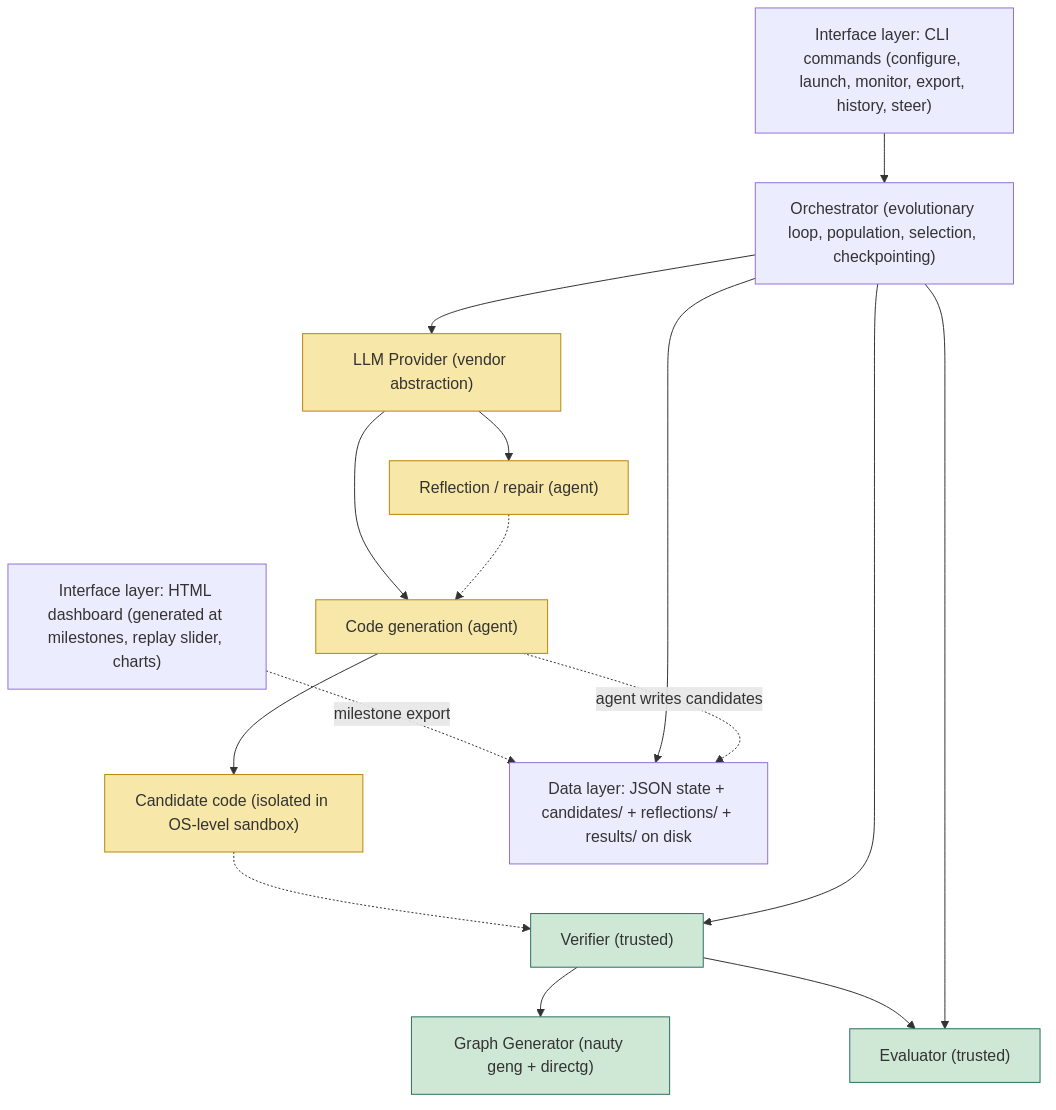
\includegraphics[width=\textwidth]{diagrams/architecture.png}
  \caption{System architecture. Yellow components are agent-driven and dynamic; green components are trusted infrastructure that agents cannot read or modify. The dashed line marks the trust boundary enforced by the OS-level sandbox (Section~\ref{sec:sandbox}).}
  \label{fig:architecture}
\end{figure}

Figure~\ref{fig:architecture} is read top to bottom. The \emph{interface} layer (CLI plus the static dashboard) is where a human launches, monitors, replays, and steers a run. The \emph{orchestration} layer owns the evolutionary loop, the population, selection, and checkpointing, and it is the only component that may invoke the verifier. The \emph{agent} layer is the untrusted zone: LLM-driven code generation, failure reflection, and repair live here and are confined to a sandbox. The \emph{verification} layer is trusted: it generates test graphs, replays operation sequences, checks invariants, and measures work. The \emph{data} layer persists runs, candidates, reflections, and results as JSON files on disk.

\subsection{Layer Responsibilities}

\begin{longtable}{|p{3cm}|p{6cm}|p{4.5cm}|}
\hline
\textbf{Layer} & \textbf{Responsibility} & \textbf{Trust level} \\
\hline
\endfirsthead
\hline
\textbf{Layer} & \textbf{Responsibility} & \textbf{Trust level} \\
\hline
\endhead
\hline
\endfoot

Interface & CLI commands and the static HTML dashboard (launch, monitor, replay, steer, export) & Neutral \\
\hline
Orchestration & Evolutionary loop, population management, selection, checkpointing, verifier invocation & Neutral \\
\hline
Agent & Code generation, failure analysis, repair; runs in an OS sandbox & Dynamic (untrusted) \\
\hline
Verification & Correctness testing (invariant), efficiency measurement, graph enumeration & Trusted (pre-built) \\
\hline
Data & Persistence, file formats, run/candidate schema, atomic writes & Neutral \\
\hline
\end{longtable}

\subsection{Principal Data and Control Flow}

The control flow of one run is:

\begin{enumerate}[noitemsep]
  \item The user configures a run via CLI (problem, provider, model, population size, generation budget, verification bound) and the configuration is validated and saved as YAML.
  \item The orchestrator either loads a previous checkpoint (resume) or initializes an empty population.
  \item For each generation:
  \begin{enumerate}[label=\alph*)]
    \item The orchestrator selects parents from the population (elitism plus diversity).
    \item The agent generates new candidates inside the sandbox; each candidate is written to the candidate store.
    \item The orchestrator runs the trusted verifier on each candidate (the agent never sees or touches test code).
    \item For each failing candidate, the agent produces a structured reflection.
    \item The evaluator computes fitness and work ratio.
    \item The orchestrator updates the population, commits the generation atomically, and (every $N$ generations, default 10) emits a dashboard snapshot.
  \end{enumerate}
  \item On a stop condition (fitness $= 1.0$ within bound, or max generations), results are exported.
\end{enumerate}

The data flow is unidirectional across the trust boundary: candidates (code) flow \emph{in} to the sandbox; structured test results (pass/fail, failing case, work ratio) flow \emph{out} to the orchestrator. The verifier's source, its test graphs, and its oracles are never exposed to the agent.

\subsection{Interface Separation}

A critical design decision separates \textbf{dynamic components} (agent-driven, potentially incorrect) from \textbf{trusted components} (pre-built, validated):

\begin{itemize}[noitemsep]
  \item \textbf{Dynamic:} code generation, failure reflection, candidate repair. Performed by LLM agents; may produce incorrect or malicious output.
  \item \textbf{Trusted:} verification engine, graph generation, invariant checking, oracles. Pre-built and validated against known-correct and known-bad implementations before any run. No agent can read or modify these.
\end{itemize}

This boundary is load-bearing: the validity of the entire thesis depends on the verifier being trustworthy. Section~\ref{sec:sandbox} explains how the boundary is enforced by the operating system rather than by convention.

\subsection{Deployment and Sandbox}

Figure~\ref{fig:deployment} shows the deployment view with process boundaries and sandbox isolation.

\begin{figure}[htbp]
  \centering
  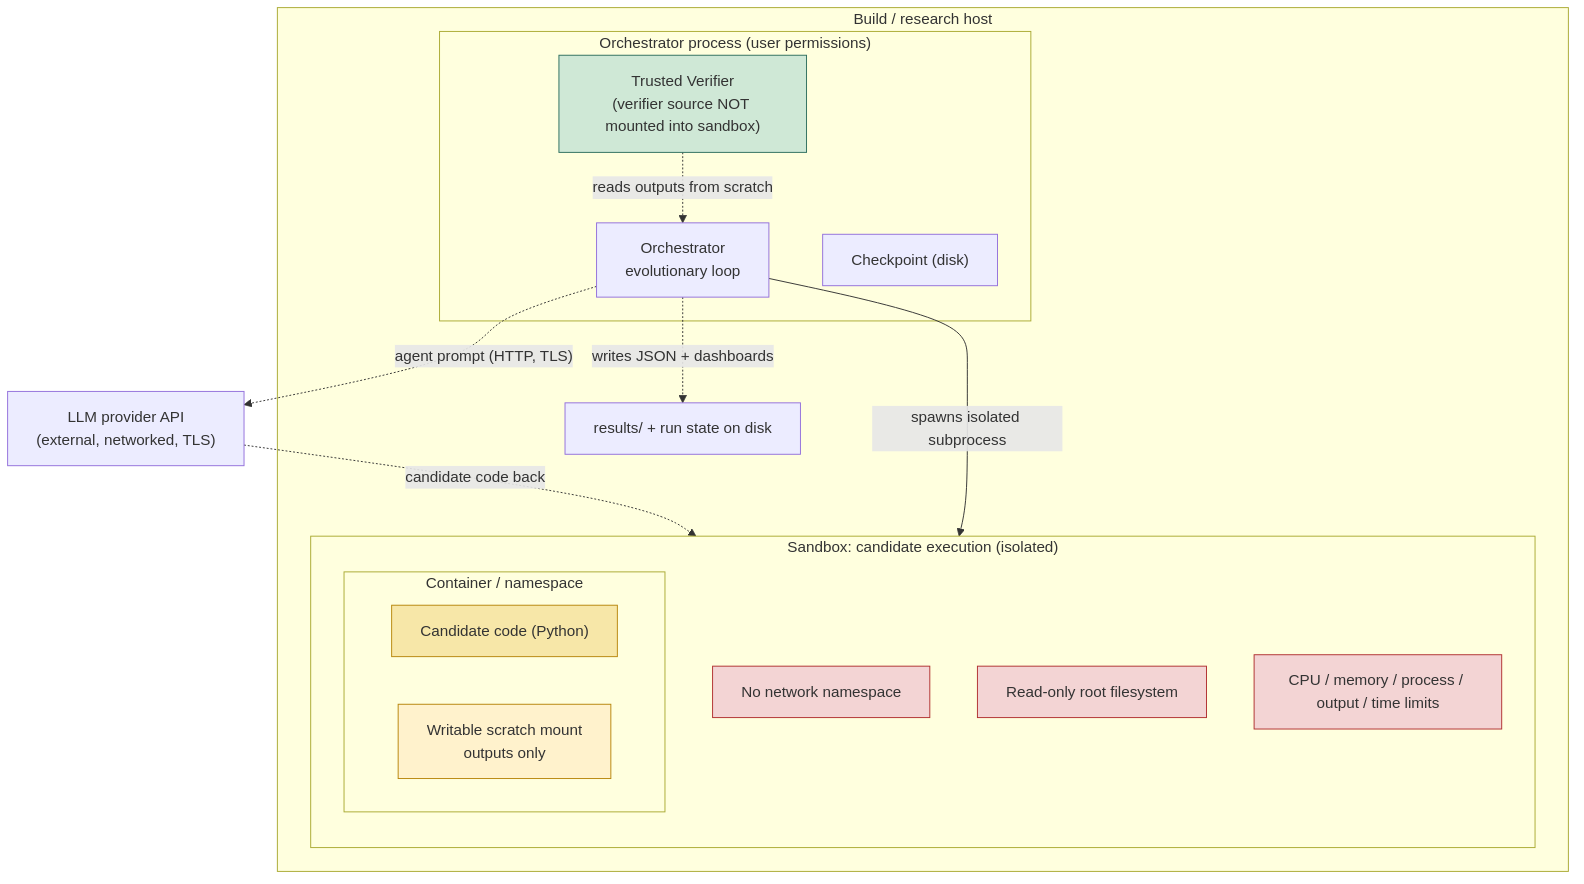
\includegraphics[width=\textwidth]{diagrams/deployment.png}
  \caption{Deployment view: the orchestrator process, the LLM provider (external, networked), and the OS-level sandbox in which untrusted candidate code executes. The sandbox has a disabled network namespace, a read-only root filesystem, no access to the verifier, and a dedicated writable scratch mount.}
  \label{fig:deployment}
\end{figure}

\subsubsection{Process Boundaries}

\begin{itemize}[noitemsep]
  \item \textbf{Orchestrator process:} a Python runtime that manages the evolutionary loop, population, evaluation, and persistence. Runs under the user's normal identity.
  \item \textbf{Agent / LLM provider:} model calls are made over HTTP by an adapter (Section~\ref{sec:provider}). Network access is required for the provider; API keys are held in environment variables, never in code or in the candidate store.
  \item \textbf{Sandbox:} candidate code executes inside a real OS isolation boundary (Section~\ref{sec:sandbox}), not in a plain subprocess.
  \item \textbf{Verifier:} trusted Python code, not generated by any LLM. It runs in the orchestrator's trust domain and is never mounted into the sandbox.
\end{itemize}

\subsubsection{Permissions}

\begin{longtable}{|p{3cm}|p{5cm}|p{5cm}|}
\hline
\textbf{Component} & \textbf{Can read} & \textbf{Can write} \\
\hline
\endfirsthead
\hline
\textbf{Component} & \textbf{Can read} & \textbf{Can write} \\
\hline
\endhead
\hline
\endfoot

Orchestrator & Run store, candidate store, verifier source & Run store, results, dashboard \\
\hline
Agent / LLM & (none of the verifier) & Sandbox scratch only \\
\hline
Candidate code & Sandbox scratch, standard libraries & Sandbox scratch only \\
\hline
Verifier & Test graphs, oracles, candidate output & Results directory \\
\hline
\end{longtable}

\label{sec:sandbox}
\subsubsection{Real OS Isolation (Not a Subprocess Env Block)}

The pre-audit design claimed that a restricted \texttt{subprocess} environment blocks network access and limits file writes. That is false: the \texttt{env} mapping of \texttt{subprocess} controls environment variables only and is not a security boundary. This design replaces it with an actual OS isolation mechanism.

The sandbox is a rootless container or namespace (for example a \texttt{unshare}d environment or a container runtime) with the following properties, each of which is a named, testable requirement:

\begin{itemize}[noitemsep]
  \item \textbf{Non-root identity:} the candidate process runs as an unprivileged user with no capability to escalate.
  \item \textbf{Disabled network namespace:} no network interfaces are available inside the sandbox; the provider call is made by the orchestrator \emph{outside} the sandbox, so the candidate never sees the API key or the network.
  \item \textbf{Read-only root filesystem:} the image is mounted read-only; the candidate cannot modify system files.
  \item \textbf{Verifier not mounted:} the verifier source, its test graphs, and its oracles are absent from the sandbox filesystem.
  \item \textbf{Dedicated writable scratch:} a single empty, writable directory is the only place the candidate may write.
  \item \textbf{Resource limits:} CPU time, memory, process count, and output size are capped by the kernel (cgroups / rlimits); a wall-clock timeout is enforced by the orchestrator.
\end{itemize}

The agent's workspace is separate from the trusted verifier, and the two communicate only through a narrow, structured interface: the orchestrator hands the sandbox a candidate file and a fixed set of inputs, and receives back a structured result record (Section~\ref{sec:verification}).

\textbf{Negative tests.} The sandbox is accepted only when the following negative tests fail as expected: a network connection attempt is refused; a write to the verifier path is refused (the path does not exist); a filesystem escape (writing outside scratch) is refused; a process-explosion attempt is killed by the process limit; an excessive-output attempt is capped; and a timeout overrun is killed by the wall-clock limit. These negative tests are part of the tool-correctness evidence (claim 1) and are listed in the traceability matrix (Table~\ref{tab:trace}).

% ============================================================
\section{Business Rules}
\label{sec:business}

\subsection{Invariants by Problem}
\label{sec:invariants}

Each problem has a correctness invariant that must hold after every operation. The pre-audit DFS and LBFS predicates were incorrect and are replaced here. The audit's own counterexample is the design's test case: in the digraph with edges $r \to a$, $a \to b$, $r \to b$, the edge $r \to b$ is a \emph{valid forward edge} even though $b$ is not a child of $r$. Any invariant that forbids forward edges would wrongly reject a correct DFS forest.

\begin{longtable}{|p{2.6cm}|p{8.2cm}|p{3.6cm}|}
\hline
\textbf{Problem} & \textbf{Invariant (corrected)} & \textbf{Verification procedure} \\
\hline
\endfirsthead
\hline
\textbf{Problem} & \textbf{Invariant (corrected)} & \textbf{Verification procedure} \\
\hline
\endhead
\hline
\endfoot

Dynamic BFS (directed) & Let $T$ be the output tree and $\delta(v)$ the distance from the root $r$ in the current graph. Then: (1) $T$ is connected and spans every vertex reachable from $r$; (2) every non-root $v$ has exactly one parent $p$ in $T$; (3) $\delta(p) = \delta(v) - 1$. & Reconstruct distances from $T$ and compare with a BFS distance oracle on the current graph; check parent uniqueness and reachability span. \\
\hline
Dynamic DFS (directed) & The output forest $T$ is a valid DFS forest of the current graph. The pre-audit ``no forward-cross edge'' predicate is \emph{not} used, because directed DFS legitimately admits forward edges. Instead $T$ is verified against a DFS-forest certificate (parent pointers plus discovery order) using the characterization of valid DFS forests in \cite{yang2019dynamic}; the verifier's predicate is validated against a certified reference implementation before any run. & Check the certificate: the parent pointers and discovery order of $T$ are consistent with a DFS of the current graph per \cite{yang2019dynamic}. Back edges are permitted and expected; forward edges are permitted; the certificate test rejects only forests that no DFS could produce. \\
\hline
Dynamic MCS (undirected) & The output is a vertex ordering that is a valid MCS ordering of the current graph: each vertex is chosen when its cardinality (number of already-chosen neighbors) is maximal among the unchosen vertices, for the stated tie-breaking. Equivalently, for chordal inputs the ordering is a perfect elimination ordering (PEO). & Check the MCS definition directly: replay the ordering and confirm each chosen vertex had maximum cardinality. Separately, for chordal inputs, run the classic $O(n+m)$ PEO check (later neighbors of each vertex form a clique) \cite{tarjan1984mcs,heggernes2006}. \\
\hline
Dynamic SCC (directed) & The output partitions vertices into sets $C_1, \ldots, C_k$ such that: (1) within each $C_i$, every vertex reaches every other via edges inside $C_i$; (2) the sets are disjoint; (3) they cover all vertices; (4) each $C_i$ is maximal \cite{karczmarz2024dynamic}. & For each $C_i$, run a reachability check both ways on the induced subgraph; verify disjointness, coverage, and maximality (no proper superset is internally mutually reachable). \\
\hline
Dynamic LBFS (directed) & The output is a total ordering $\pi$ that is a valid lexicographic BFS ordering \cite{rose1976algorithmic}. The pre-audit ``consecutive earlier neighbors'' rule is \emph{not} used, because it fails on ordinary valid LexBFS orderings (for example a four-cycle). & Verify $\pi$ against the LexBFS cone / interval characterization of \cite{rose1976algorithmic} using a reference LexBFS implementation as oracle, rather than an ad-hoc neighbor-consecutiveness predicate. \\
\hline
Reachability (directed) & For a fixed source $s$, the maintained set $R$ of vertices reachable from $s$ equals the true reachability set of the current graph \cite{demetrescu2005dynamic,bernstein2023}. & After each update, compare $R$ against a transitive-closure / reachability oracle on the current graph. \\
\hline
\end{longtable}

\textbf{Ownership.} Each invariant is owned by the \emph{Problem Definition} class, which also owns the corresponding verification procedure and oracle. The \emph{Verifier} executes the procedure but does not define it. This keeps the predicate and its enforcement in one place.

\textbf{Why invariants, not reference equality.} Dynamic outputs are non-unique: two valid BFS or DFS algorithms on the same graph may produce different trees. Judging by the invariant (a) prevents false negatives (rejecting correct algorithms), (b) catches real errors (a violated property), and (c) applies uniformly across problems. This follows the separation of discovery and verification used in LLM-driven program search \cite{openai2025codex,funsearch2023,alphaevolve2025}.

\subsection{Candidate State Machine}

The pre-audit document had three conflicting accounts of candidate state (a state table, a ``timeout = CRASH'' note, and a section that recorded timeout as FAIL). This design uses \textbf{one} state machine with explicit transition guards and terminal states.

\begin{center}
\renewcommand{\arraystretch}{1.2}
\begin{tabular}{|l|p{7.5cm}|c|}
\toprule
\textbf{State} & \textbf{Meaning} & \textbf{Terminal} \\
\midrule
\texttt{NEW} & Generated, not yet tested & No \\
\texttt{TESTING} & Under verification in the sandbox & No \\
\texttt{PASS} & Invariant held on every test sequence within bound & Yes \\
\texttt{FAIL} & At least one invariant violation, \emph{or} a timeout (recorded with a \texttt{timeout} flag) & Yes \\
\texttt{CRASH} & Runtime exception, syntax error, or sandbox resource violation & Yes \\
\texttt{DISCARDED} & Removed from the population after selection & Yes \\
\bottomrule
\end{tabular}
\end{center}

\textbf{Transition guards.}

\begin{itemize}[noitemsep]
  \item \texttt{NEW} $\to$ \texttt{TESTING}: the candidate file parses as valid Python and the sandbox accepts it.
  \item \texttt{TESTING} $\to$ \texttt{PASS}: every test sequence in the bound satisfies the invariant.
  \item \texttt{TESTING} $\to$ \texttt{FAIL}: at least one sequence violates the invariant, or the wall-clock timeout fires (state \texttt{FAIL}, flag \texttt{timeout=true}).
  \item \texttt{TESTING} $\to$ \texttt{CRASH}: an exception, a syntax error, or a sandbox limit (process, memory, output) is hit.
  \item \texttt{PASS} / \texttt{FAIL} / \texttt{CRASH} $\to$ \texttt{DISCARDED}: selection removes the candidate from the population.
\end{itemize}

The rule is fixed and unambiguous: \textbf{timeout maps to \texttt{FAIL} with a timeout flag; a crash maps to \texttt{CRASH}.} The state, the JSON schema, the dashboard, and the recovery logic all use this single table.

\subsection{Failure Policies}

\begin{itemize}[noitemsep]
  \item \textbf{Timeout:} each candidate execution runs under a configurable wall-clock timeout (default 30 s). Non-termination is recorded as \texttt{FAIL} with \texttt{timeout=true} and the run continues.
  \item \textbf{Crash / sandbox violation:} recorded as \texttt{CRASH}; the run continues.
  \item \textbf{LLM provider failure:} transient API failures are retried up to 3 times with exponential backoff; if still failing, the candidate slot is left empty for that generation and the failure is logged.
  \item \textbf{All candidates fail:} a warning is logged and the loop continues to the next generation (diversity mutation may recover).
  \item \textbf{Candidate isolation:} generated code is untrusted and runs only in the sandbox; a crash never halts the run.
\end{itemize}

\subsection{Input Validation}

\begin{itemize}[noitemsep]
  \item \textbf{Graph size:} $n \geq 1$. Exhaustive verification for $n \le 5$; sampling for $n > 5$.
  \item \textbf{Population size:} $1 \le \texttt{pop\_size} \le 50$, default 10.
  \item \textbf{Max generations:} $1 \le \texttt{max\_gen} \le 1000$, default 100.
  \item \textbf{Model name:} must be a valid identifier in the configured provider; validated at configuration time.
  \item \textbf{Timeout:} $1 \le \texttt{timeout} \le 300$ s, default 30.
  \item \textbf{Candidate code:} must be valid Python; a syntax error is recorded as \texttt{CRASH}.
\end{itemize}

\subsection{Domain Rules and Their Enforcement}

\begin{longtable}{|p{4.5cm}|p{5.5cm}|p{4.5cm}|}
\hline
\textbf{Rule} & \textbf{Content} & \textbf{Enforced by} \\
\hline
\endfirsthead
\hline
\textbf{Rule} & \textbf{Content} & \textbf{Enforced by} \\
\hline
\endhead
\hline
\endfoot

Adjacency-matrix representation & All graphs are simple, loop-free $0/1$ matrices; legal updates flip one entry. & Problem Definition \\
\hline
Legal operations & Only insert/delete of a single matrix entry; no structural mutation. & Verifier (sequence generator) \\
\hline
Invariant ownership & One invariant + oracle per problem. & Problem Definition \\
\hline
Trust boundary & Agents cannot read/modify verifier or its inputs. & Sandbox (OS) \\
\hline
State discipline & Single state machine, timeout=FAIL, crash=CRASH. & Orchestrator \\
\hline
Efficiency threshold & $\text{work\_ratio} < 1$ required for an improvement. & Evaluator \\
\hline
Bounded claims & No ``proof'' language without a stated bound. & Author / review \\
\hline
\end{longtable}

% ============================================================
\section{Class Design}
\label{sec:class}

\subsection{Class Diagram}

Figure~\ref{fig:classes} shows the twelve core classes, their associations, multiplicities, ownership, and key operations.

\begin{figure}[htbp]
  \centering
  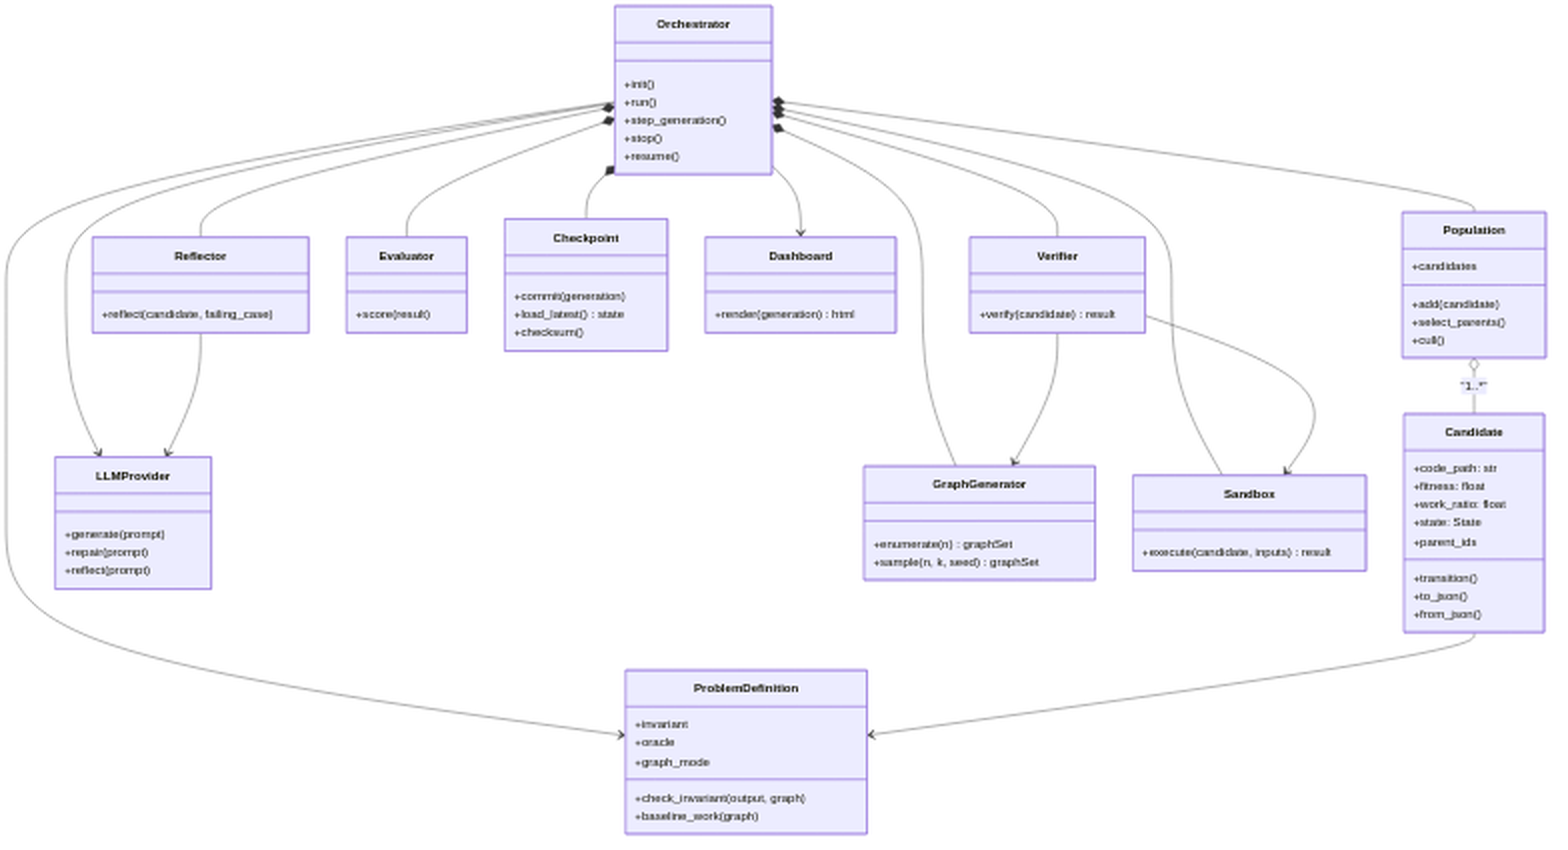
\includegraphics[width=\textwidth]{diagrams/classes.png}
  \caption{Class diagram of the twelve core classes with associations, multiplicities, ownership (composition shown by filled diamond), and key operations. The Orchestrator composes the Population, Verifier, Reflector, Evaluator, Graph Generator, Sandbox, and Checkpoint; it uses the LLM Provider, Problem Definition, and Dashboard.}
  \label{fig:classes}
\end{figure}

Figure~\ref{fig:classes} is the mandatory class diagram. The \emph{Orchestrator} is the composition root: it owns (filled diamond) the \texttt{Population}, \texttt{Verifier}, \texttt{Reflector}, \texttt{Evaluator}, \texttt{GraphGenerator}, \texttt{Sandbox}, and \texttt{Checkpoint}, and it uses (open arrow) the \texttt{LLMProvider}, \texttt{ProblemDefinition}, and \texttt{Dashboard}. The \texttt{Population} aggregates \texttt{Candidate} instances (multiplicity $1..*$). The \texttt{Verifier} uses the \texttt{GraphGenerator} to enumerate test graphs and the \texttt{Sandbox} to execute candidates. The \texttt{Reflector} and the \texttt{LLMProvider} are associated: the reflector issues structured prompts through the provider. The \texttt{Candidate} holds a lineage list of parent ids and a state from the single state machine.

\subsection{The Twelve Core Classes}

\begin{longtable}{|p{3cm}|p{10cm}|}
\hline
\textbf{Class} & \textbf{Responsibility and key operations} \\
\hline
\endfirsthead
\hline
\textbf{Class} & \textbf{Responsibility and key operations} \\
\hline
\endhead
\hline
\endfoot

Orchestrator & Composition root. Drives the evolutionary loop; coordinates all components from initialization to completion. Key operations: \texttt{init()}, \texttt{run()}, \texttt{step\_generation()}, \texttt{stop()}, \texttt{resume()}. Owns the population and delegates verification, reflection, evaluation, and checkpointing. \\
\hline
Population & Manages the candidate collection. Key operations: \texttt{add()}, \texttt{select\_parents()}, \texttt{cull()}. Enforces population size, elitism, and diversity. \\
\hline
Candidate & One algorithm attempt. Stores code path, fitness, work ratio, state (single state machine), generation, \texttt{parent\_ids} (multi-parent lineage), and reflection text. Key operations: \texttt{transition()}, \texttt{to\_json()}, \texttt{from\_json()}. \\
\hline
LLM Provider & Vendor-agnostic abstraction for model access (adapter pattern). Key operations: \texttt{generate()}, \texttt{repair()}, \texttt{reflect()}. One concrete adapter is OpenCode; API keys come from the environment. \\
\hline
Verifier & Trusted correctness and efficiency tester. Key operations: \texttt{verify(candidate)} $\to$ result record. Generates test graphs, replays operation sequences, checks the invariant after each operation, and measures work. Never exposed to the agent. \\
\hline
Reflector & Analyzes failed candidates and produces structured reflections (failure description, root cause, repair hints) reused as repair context. Key operations: \texttt{reflect(candidate, failing\_case)}. \\
\hline
Evaluator & Computes fitness (fraction of sequences passing) and work ratio ($\text{candidate\_work}/\text{offline\_work}$); applies the $<1$ improvement threshold. Key operations: \texttt{score(result)}. \\
\hline
Problem Definition & Encapsulates one problem (BFS, DFS, MCS, SCC, LBFS, reachability). Owns the invariant, the oracle, the tie-breaking rule, and the efficiency baseline. Key operations: \texttt{check\_invariant(output, graph)}, \texttt{baseline\_work(graph)}. \\
\hline
Graph Generator & Wraps the nauty tools (\texttt{geng} + \texttt{directg}). Enumerates all non-isomorphic digraphs up to size $n$ and produces random samples beyond. Key operations: \texttt{enumerate(n)} $\to$ graph set, \texttt{sample(n, k, seed)} $\to$ graph set. \\
\hline
Checkpoint & Persistence. Key operations: \texttt{commit(generation)} (atomic temp-write + rename), \texttt{load\_latest()} (resume), \texttt{checksum()}. Owns run ids, schema version, retention, and partial-generation recovery. \\
\hline
Sandbox & OS-level isolation boundary. Key operations: \texttt{execute(candidate, inputs)} $\to$ structured result. Enforces non-root identity, disabled network, read-only root fs, no verifier mount, scratch-only writes, and CPU/memory/process/output/time limits. \\
\hline
Dashboard & Static HTML output. Key operations: \texttt{render(generation)} $\to$ self-contained HTML. Emits every $N$ generations (default 10, configurable) with client-side interactivity: overview, generation replay, candidate detail, failure reflections, config. \\
\hline
\end{longtable}

\textbf{Correspondence to responsibilities.} The orchestration layer is \texttt{Orchestrator} + \texttt{Population}; the agent layer is \texttt{LLMProvider} + \texttt{Reflector} (confined by \texttt{Sandbox}); the verification layer is \texttt{Verifier} + \texttt{ProblemDefinition} + \texttt{GraphGenerator} + \texttt{Evaluator}; the data layer is \texttt{Checkpoint} + \texttt{Candidate}; the interface layer is the CLI (in \texttt{Orchestrator}) + \texttt{Dashboard}. No class is orphaned and no named responsibility lacks a class.

% ============================================================
\section{Data Design}
\label{sec:data}

\subsection{Storage Choice}

All state is persisted to the local filesystem as JSON files plus the candidate Python files themselves. No database is used. The reasons are project-specific: the data model is small and hierarchical (runs $\to$ generations $\to$ candidates), a researcher needs to inspect state by hand, and portability to any Python host is a stated non-functional requirement. A relational store would add setup, a schema migration story, and a server dependency for no query benefit at this scale.

\subsection{Directory Layout}

\begin{verbatim}
project/
  runs/
    <run_id>/
      config.yaml            # validated run configuration
      generation_0001.json   # committed generation state
      generation_0002.json
      ...
      COMMITTED              # marker: last fully committed generation
      candidates/
        gen001_c01.py        # generated code
        ...
      reflections/
        gen001_c01.md        # structured failure analyses
        ...
      dashboard/
        gen0010.html         # snapshot every N generations
        ...
      results/
        run_summary.json
        efficiency_report.csv
  graphs/
    n4/                      # cached nauty graphs (size 4)
    n5/
    ...
\end{verbatim}

\subsection{Entities and Relationships}

The persistence entities are \textbf{Run}, \textbf{Generation}, \textbf{Candidate}, \textbf{Reflection}, and \textbf{Result}. A Run has many Generations (ordered by number). A Generation has many Candidates. A Candidate has zero or one Reflection (when it failed) and one Result. A Candidate references zero or more parent Candidates by id (multi-parent lineage). The relationships are encoded as nested JSON plus id references; there are no foreign keys to enforce, so integrity is guaranteed by the single-writer rule (only the orchestrator writes, atomically).

\subsection{Generation State Schema}

The generation file \texttt{generation\_\{N\}.json} has a fixed schema version:

\begin{verbatim}
{
  "schema_version": 2,
  "run_id": "run_20260918_0001",
  "generation": 42,
  "timestamp": "2026-09-18T20:59:00Z",
  "problem": "dynamic_mcs",
  "bound": { "n_max": 5, "seq_len_max": 20, "seed": 1337 },
  "candidates": [
    {
      "id": "gen042_c03",
      "code_path": "candidates/gen042_c03.py",
      "fitness": 0.85,
      "work_ratio": 0.72,
      "state": "FAIL",
      "timeout": false,
      "parent_ids": ["gen041_c01", "gen041_c05"],
      "tests_passed": 17,
      "tests_total": 20
    }
  ],
  "config_ref": "config.yaml",
  "checksum": "sha256:..."
}
\end{verbatim}

Note the corrected example: a candidate with fitness $0.85$ and $17/20$ tests is \texttt{FAIL}, not \texttt{PASS} (the pre-audit example marked it \texttt{PASS}). \texttt{PASS} requires fitness $1.0$ within the bound. The \texttt{parent\_ids} list supports multi-parent lineage; the pre-audit schema had a single \texttt{parent\_id}.

\subsection{Candidate File Format}

Each candidate is a self-contained Python module implementing a fixed interface:

\begin{verbatim}
def init(graph):
    """Build initial state from the starting adjacency matrix."""
    ...

def insert_edge(graph, edge, state):
    """Update state after inserting edge (u, v). Returns new state."""
    ...

def delete_edge(graph, edge, state):
    """Update state after deleting edge (u, v). Returns new state."""
    ...
\end{verbatim}

The verifier calls \texttt{init} once per base graph, then replays a sequence of \texttt{insert\_edge} / \texttt{delete\_edge}, checking the invariant after each call.

\subsection{Constraints, Lifecycle, and Integrity}

\begin{itemize}[noitemsep]
  \item \textbf{Run id:} unique per run, generated at \texttt{init()} (timestamp + counter). It namespaces all files so parallel runs never collide.
  \item \textbf{Candidate id:} unique within a run as \texttt{gen\{N\}\_c\{M\}}; enforced by the population.
  \item \textbf{Schema version:} \texttt{schema\_version} is read on load; an incompatible version is rejected with a clear error (compatibility rule), never silently migrated.
  \item \textbf{Atomicity:} a generation is written to a temporary file and then renamed over the target (\texttt{os.replace}), which is atomic on POSIX. The \texttt{COMMITTED} marker is written only after the rename succeeds. A crash mid-write leaves either the old complete file or the new complete file, never a torn file.
  \item \textbf{Checksum:} each generation file carries a SHA-256 of its content; on load the checksum is verified, and a mismatch is treated as corruption.
  \item \textbf{Partial-generation recovery:} on resume, the orchestrator reads \texttt{COMMITTED} to find the last complete generation and discards any incomplete file beyond it.
  \item \textbf{Retention:} generation files are retained by default; an optional retention policy can prune old generations while always keeping the last committed one and the run summary.
  \item \textbf{Concurrency:} single-writer. Only the orchestrator process writes to a run directory; the dashboard is read-only.
\end{itemize}

\subsection{Interfaces}

The data layer exposes \texttt{Checkpoint.commit(generation)}, \texttt{Checkpoint.load\_latest(run\_id)}, \texttt{Checkpoint.checksum(path)}, and the \texttt{Candidate.to\_json} / \texttt{from\_json} pair. The CLI and dashboard read through these; they never write raw JSON.

% ============================================================
\section{Interaction Design}

\subsection{Interface Model}

The registered contribution 1 is an interactive platform that launches, monitors, replays, and steers a run. This design delivers that as a \textbf{CLI engine plus milestone HTML dashboards}. The CLI is the control plane (launch, configure, steer, export); the dashboard is the observation and replay plane (self-contained static HTML with client-side interactivity). This is a faithful realization of the registered UI, not a replacement by CLI alone: the dashboard provides the launch/monitor/replay visualization and the CLI provides the steering.

\subsection{CLI Commands}

\begin{longtable}{|p{4cm}|p{10cm}|}
\hline
\textbf{Command} & \textbf{Description} \\
\hline
\endfirsthead
\hline
\textbf{Command} & \textbf{Description} \\
\hline
\endhead
\hline
\endfoot

\texttt{run configure} & Set and validate run parameters (problem, provider, model, population, generations, bound, timeout); writes \texttt{config.yaml}. \\
\hline
\texttt{run start} & Begin the evolutionary loop for a configured run. \\
\hline
\texttt{run status} & Show current generation, best fitness, pass rate, and failure patterns. \\
\hline
\texttt{run steer} & Inject a steering directive (e.g., change model, bias diversity, set a new bound) into the next generation via a YAML patch. \\
\hline
\texttt{run stop} & Gracefully stop after the current generation commits. \\
\hline
\texttt{run resume} & Reload the last committed generation and continue. \\
\hline
\texttt{run export} & Save results as a human-readable report and structured data. \\
\hline
\texttt{run history} & List previous runs with summaries. \\
\hline
\end{longtable}

\subsection{Dashboard Views, Navigation, and Handlers}

The dashboard is emitted every $N$ generations (default 10, configurable) as a single self-contained static HTML file (embedded data, client-side JavaScript, no server). It has five views, navigable by a top bar:

\begin{longtable}{|p{3.5cm}|p{6cm}|p{4.5cm}|}
\hline
\textbf{View} & \textbf{Content} & \textbf{Primary handler} \\
\hline
\endfirsthead
\hline
\textbf{View} & \textbf{Content} & \textbf{Primary handler} \\
\hline
\endhead
\hline
\endfoot

Overview & Run id, problem, bound, current generation, best fitness, stop status & \texttt{renderOverview()} \\
\hline
Generation replay & Fitness chart over generations; a slider scrubs through generations and re-renders the population at that generation & \texttt{onSlider(g)} \\
\hline
Candidate detail & One candidate's code path, state, fitness, work ratio, parent lineage, and per-sequence results & \texttt{openCandidate(id)} \\
\hline
Failure reflections & List of failing candidates with their structured reflections (description, root cause, repair hints) & \texttt{openReflection(id)} \\
\hline
Config & The validated \texttt{config.yaml} and the verification bound & \texttt{renderConfig()} \\
\hline
\end{longtable}

The replay slider is the key interaction: it lets the user scrub a multi-generation run forward and backward, which is exactly the registered ``replay'' completion signal. Steering is done from the CLI (\texttt{run steer}) between generations, not inside the dashboard, keeping the dashboard read-only and the control plane explicit.

\subsection{Input, Output, and Request Flow}

\begin{itemize}[noitemsep]
  \item \textbf{Input:} a YAML configuration (CLI) and, optionally, a steering patch (\texttt{run steer}).
  \item \textbf{Output:} real-time terminal progress; per-generation JSON; milestone HTML dashboards; a final \texttt{run\_summary.json} and \texttt{efficiency\_report.csv}.
  \item \textbf{Request flow (launch):} \texttt{run configure} validates and saves config $\to$ \texttt{run start} initializes or resumes $\to$ the loop steps generations, committing each and emitting a dashboard every $N$.
\end{itemize}

\subsection{Error Behavior}

\begin{itemize}[noitemsep]
  \item \textbf{Invalid configuration:} rejected at \texttt{run configure} with a named field and allowed range; no run is started.
  \item \textbf{Provider failure:} retried up to 3 times with backoff; then the candidate slot is left empty and the failure is logged.
  \item \textbf{Candidate crash / timeout:} recorded as \texttt{CRASH} / \texttt{FAIL}+timeout per the single state machine; the run continues.
  \item \textbf{Corrupt checkpoint:} checksum mismatch or incompatible \texttt{schema\_version} is reported and the run refuses to resume until the user resolves it.
  \item \textbf{All candidates fail:} a warning is logged and the loop continues.
\end{itemize}

% ============================================================
\section{Core Logic and Scientific Model}
\label{sec:corelogic}

\subsection{Evolutionary Loop}

Figure~\ref{fig:loop} shows the evolutionary loop as a sequence diagram.

\begin{figure}[htbp]
  \centering
  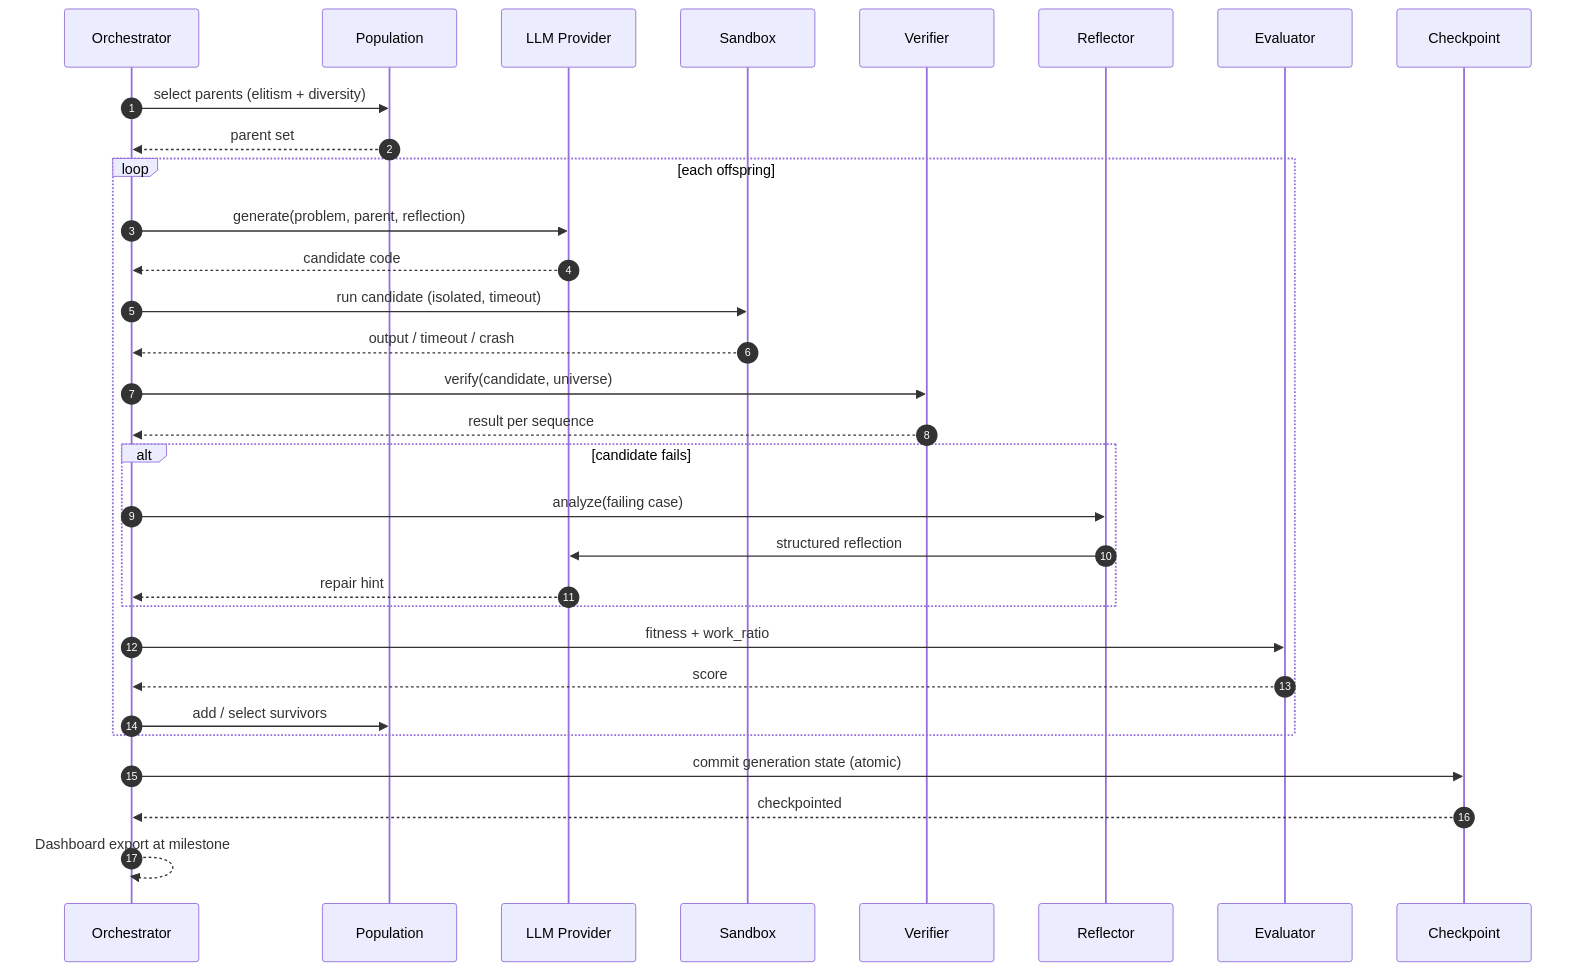
\includegraphics[width=\textwidth]{diagrams/loop.png}
  \caption{Evolutionary loop sequence diagram: the Orchestrator selects parents, the LLM Provider generates candidates, the Sandbox executes them under the Verifier, the Reflector produces reflections on failure, the Evaluator scores, and the Checkpoint commits each generation.}
  \label{fig:loop}
\end{figure}

The loop is implementable from the following contract.

\textbf{Inputs:} a validated config (problem, provider, model, population size, generation budget, verification bound, timeout, diversity rate, elitism $k$).

\textbf{Per generation:}
\begin{enumerate}[noitemsep]
  \item \emph{Select parents.} Keep the top-$k$ by fitness (elitism). Add parents by fitness-proportional selection. If the population's pairwise similarity exceeds a threshold, inject a diversity mutation (a fresh candidate from a new prompt, not derived from any parent).
  \item \emph{Generate offspring.} For each parent (or pair, for multi-parent), the LLM Provider is prompted with the problem interface, the parent code, and (for repair) the structured reflection. The returned code is written to the candidate store and marked \texttt{NEW}.
  \item \emph{Verify.} The Verifier runs each \texttt{NEW} candidate in the Sandbox over the bounded test universe (Section~\ref{sec:verification}); each transition follows the single state machine.
  \item \emph{Reflect.} For each \texttt{FAIL} / \texttt{CRASH} candidate, the Reflector produces a structured reflection.
  \item \emph{Score.} The Evaluator computes fitness and work ratio.
  \item \emph{Select and commit.} The Population culls to its size (worst first, preserving diversity), and the Checkpoint commits the generation atomically.
\end{enumerate}

\textbf{Stop conditions:} a candidate reaches fitness $1.0$ within the bound (success), or the generation budget is exhausted (report best-so-far).

\textbf{Invariants of the loop:} the population size never exceeds its configured maximum; every committed generation is atomic and checksummed; the verifier is invoked only by the orchestrator; no generation is committed twice.

\subsection{Verification Process}
\label{sec:verification}

Figure~\ref{fig:verification} details the verification of one candidate.

\begin{figure}[htbp]
  \centering
  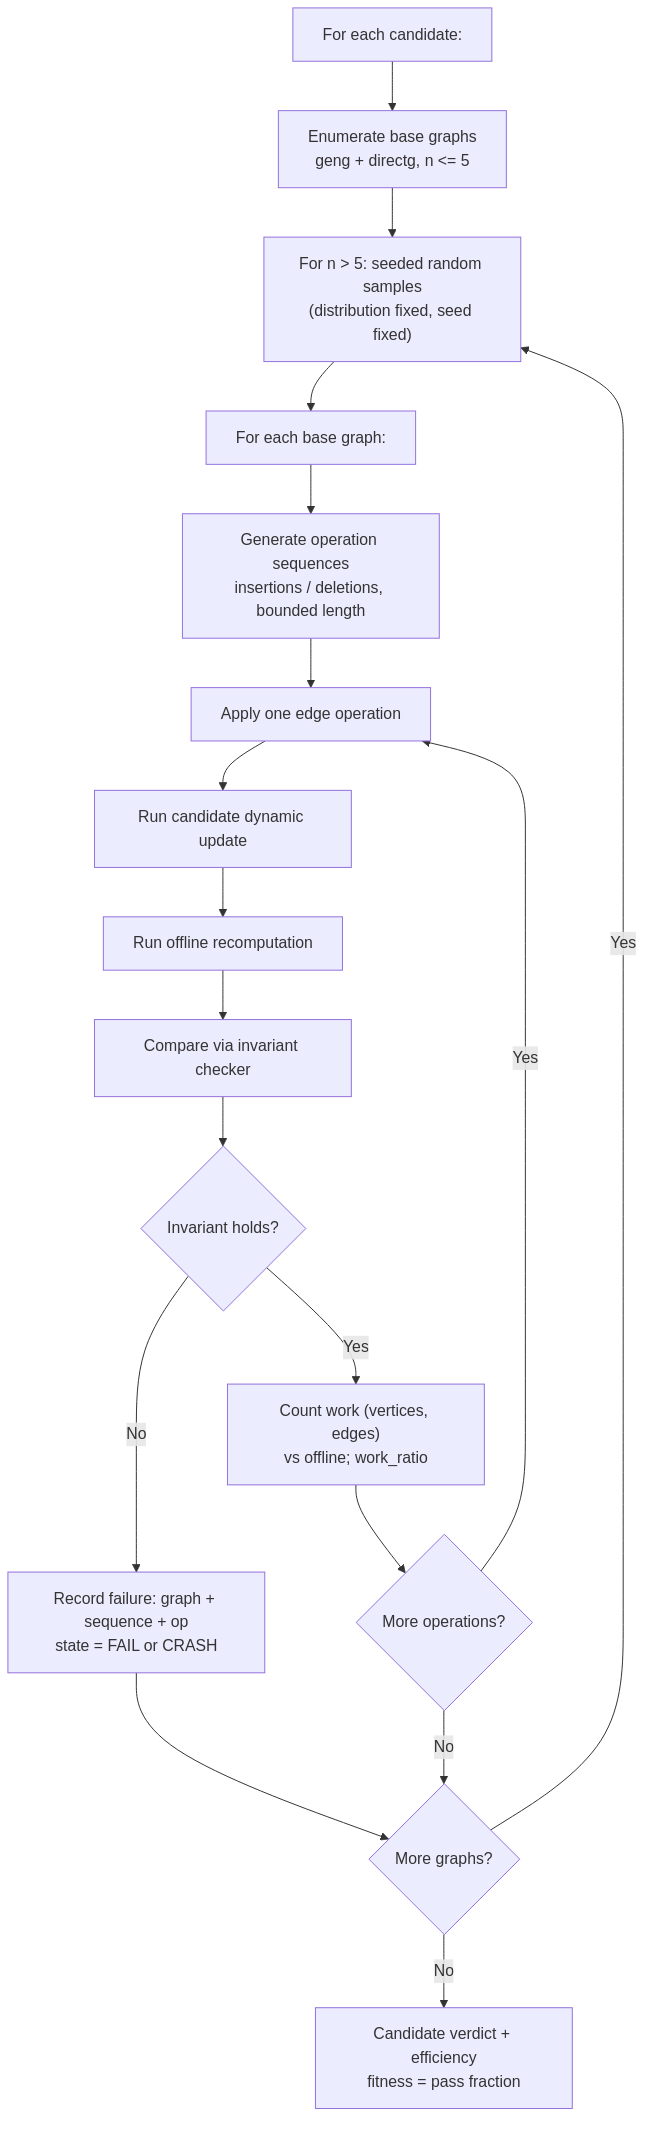
\includegraphics[width=\textwidth]{diagrams/verification.png}
  \caption{Verification flow: enumerate the bounded test universe (all non-isomorphic digraphs up to $n \le 5$ via geng + directg, plus seeded random samples beyond), and for each base graph replay operation sequences, checking the invariant after every operation and measuring work.}
  \label{fig:verification}
\end{figure}

\textbf{Test universe (finite and reproducible).}
\begin{itemize}[noitemsep]
  \item \emph{Base graphs:} all non-isomorphic digraphs up to size $n \le 5$, enumerated by nauty \texttt{geng} + \texttt{directg}. For $n > 5$, a fixed number of random graphs drawn from a stated distribution with a fixed seed.
  \item \emph{Operation sequences:} for each base graph, a bounded set of interleaved insert/delete sequences up to a stated maximum length. The bound (graph size, sequence length, sample count, seed) is part of the run config and is recorded in every result, so the claim ``no counterexample within the stated bound'' is reproducible.
  \item \emph{Invariant check:} after \emph{every} operation, the Problem Definition's invariant is checked against the oracle.
\end{itemize}

\textbf{Efficiency measurement.} The work a candidate performs (vertices visited, edges scanned, instrumented) is compared against the offline recomputation baseline for the same operation. The \texttt{work\_ratio} is $\text{candidate\_work} / \text{offline\_work}$, aggregated (median) across operations and graphs. An efficiency \emph{improvement} requires $\text{work\_ratio} < 1$; a ratio $> 1$ means the candidate does more work than simply recomputing, which is not an improvement. Wall-clock is reported separately from instrumented work.

\textbf{Bounded, not proof.} The verifier outputs ``no counterexample within the stated bound''. It does not claim correctness for arbitrary size or update length. That claim is reserved for the Lean phase.

\textbf{Verifier validation (claim 1).} Before any experiment, the verifier is validated against (a) known-good reference algorithms (for example the dynamic DFS of \cite{yang2019dynamic}) and (b) a known-bad mutation corpus (deliberately faulty edits). The acceptance target is zero false negatives for $n \le 5$: every known-bad mutation is rejected and every known-good algorithm is accepted.

\subsection{Reflection Process}
\label{sec:reflection}

When a candidate fails, the Reflector:
\begin{enumerate}[noitemsep]
  \item reads the candidate code and the failing case (graph, operation sequence, the invariant that was violated, and the oracle's expected property);
  \item traces the algorithm on the failing case;
  \item identifies the root cause (which invariant was violated, where, and what condition was unhandled);
  \item emits a structured reflection with three fields: \emph{failure description}, \emph{root cause}, and \emph{repair hints}.
\end{enumerate}
The reflection is fed into the next generation's repair prompt. This is the verbal-reinforcement mechanism of \cite{reflexion2023}, applied to code repair.

\subsection{Generative Operators and Prompt Contracts}

The evolutionary operators are concrete and implementable. Each operator is a function of the current population and the problem definition, and each produces one or more \texttt{NEW} candidates.

\textbf{Generation (mutation from a parent).} Given a parent candidate $P$, the LLM Provider is prompted with a fixed template containing: (1) the problem interface (the \texttt{init}/\texttt{insert\_edge}/\texttt{delete\_edge} contract and the invariant statement, but \emph{not} the verifier's oracle code); (2) the parent source code; (3) a directive to produce a modified candidate. The returned code is written to the store and marked \texttt{NEW}. This is the primary operator.

\textbf{Repair (reflection-driven).} Given a failing candidate $F$ and its structured reflection $R$, the LLM Provider is prompted with the same template plus $R$ (failure description, root cause, repair hints). The repair prompt is the distinguishing feature of this system: it converts a bounded counterexample into a targeted edit rather than a blind rewrite.

\textbf{Crossover (multi-parent).} Given two parents $P_1, P_2$ (both must be at least \texttt{PASS}-adjacent, i.e., not \texttt{CRASH}), the LLM Provider is prompted with both source files and a directive to combine their update strategies into one candidate. The offspring records both ids in \texttt{parent\_ids}, which is why the schema uses a list rather than a single \texttt{parent\_id}. Crossover is optional and gated by a config flag; it is off by default for the calibration problems.

\textbf{Diversity (injection).} When the population's pairwise similarity exceeds a threshold (similarity is measured as the fraction of candidates whose fitness and failing-case signature are within a small epsilon), the operator injects a fresh candidate generated from a blank template (no parent), to preserve exploration.

\textbf{Prompt schema.} Every prompt is a fixed, versioned template with named slots (problem, interface, invariant, parent code, reflection, operator). The template version is recorded in the run config so that a result is reproducible: same config, same seeds, same template version, same provider/model $\Rightarrow$ same candidate set. The agent never sees the verifier source, the test graphs, or the oracle; it sees only the interface and the invariant statement.

\subsection{Selection Strategy}

Selection determines which candidates survive to the next generation. The order is fixed:

\begin{enumerate}[noitemsep]
  \item \textbf{Elitism:} the top-$k$ by fitness (default $k=2$) are always kept, regardless of other rules.
  \item \textbf{Repair preference:} among the remaining slots, candidates with informative reflections (a \texttt{FAIL} with a non-empty root cause) are preferred for repair over fresh generation, because a targeted edit is cheaper than a blind rewrite.
  \item \textbf{Diversity:} if the similarity threshold is exceeded, one slot is reserved for a fresh (no-parent) candidate.
  \item \textbf{Cull:} the population is reduced to its configured size by removing the lowest-fitness non-elite candidates, preserving at least one distinct failing-case signature to keep exploration.
\end{enumerate}

\textbf{Stop conditions:} a candidate reaches fitness $1.0$ within the bound (success, the run stops and exports), or the generation budget is exhausted (the run stops and reports best-so-far). A plateau (below) does not stop the run; it only triggers dynamic agent generation.

\subsection{Cooperative Agents and Dynamic Agent Generation}

Registered contribution 3 is cooperative agents with optional dynamic agent generation. The design fixes the initial roles, the message protocol, the plateau detector, and the dynamic-generation rule, so the principal modules are implementable; the cooperation \emph{policy} (cooperative vs.\ critical, and whether dynamic generation helps) is the empirical research question decided from the first experiments, as the SRS states.

\textbf{Initial roles.}
\begin{itemize}[noitemsep]
  \item \emph{Generator:} proposes new candidate code from a parent (or blank) and the problem interface.
  \item \emph{Reflector / critic:} reads a failing case and produces the structured reflection.
  \item \emph{Orchestrator (coordinator):} the only component that routes artifacts between agents and invokes the verifier. Agents never call each other directly.
\end{itemize}

\textbf{Message protocol.} Agents exchange only structured artifacts through the orchestrator: a \emph{candidate} (code + id + parent ids), a \emph{failing case} (graph, operation sequence, violated invariant, oracle property), and a \emph{reflection} (description, root cause, repair hints). Each artifact has a fixed schema (Section~\ref{sec:reflection}) and an id, so the full transcript is logged and reproducible.

\textbf{Plateau detection.} A plateau is declared when the best fitness over a sliding window of $W$ generations (default $W=10$) improves by less than a threshold $\epsilon$ (default $0.01$). The window and threshold are config parameters.

\textbf{Dynamic agent generation.} On a plateau, the system may spawn an additional specialized agent whose prompt is biased toward the most frequent failing-case signature in the window (for example, an agent that focuses on the specific invariant clause that keeps failing). Spawning is bounded by an \emph{agent budget} (maximum concurrent agents, default 3) and a \emph{generation budget} for each spawned agent. A spawned agent is retired when (a) the budget is exhausted, or (b) it has not contributed a fitness improvement in $W$ generations. Baselines for comparison: a single-agent run and a fixed two-agent (generator + reflector) run, all under equal model-call and generation budgets.

\textbf{Budgets.} Every run has a model-call budget (maximum LLM invocations) and a generation budget (maximum generations). The orchestrator enforces both; exceeding either stops the run and exports best-so-far. Budgets make negative results comparable and reproducible.

% ============================================================
\section{Design Rationale and Alternatives}
\label{sec:rationale}

\subsection{CLI Engine Plus Dashboard, Not a Web App}

The registered UI is realized as a CLI control plane plus self-contained static HTML dashboards. Alternatives considered: (a) a full web application with a server, and (b) CLI only. A web app adds a server, a build pipeline, and a deployment target that a single-researcher tool does not need, and it complicates reproducibility. CLI only would drop the registered replay/visualization promise. The CLI+dashboard split keeps the control plane scriptable and version-controllable (reproducible experiments) while delivering launch, monitor, replay, and visualization as static artifacts that need no server.

\subsection{Orchestrator-Run Verification}

The verifier is invoked by the orchestrator, not by the agent. Alternatives: letting the agent run its own tests. That would let the agent modify or skip tests, breaking the trust boundary on which the thesis rests. Orchestrator-run verification guarantees that the same candidate always produces the same result regardless of agent behavior, and it keeps the verifier source out of the agent's reach.

\subsection{Correctness by Invariant}

Dynamic outputs are non-unique, so reference equality would produce false negatives. Alternatives: canonicalizing outputs (fragile, problem-specific) or comparing to one offline oracle tree (rejects valid alternatives). Invariant checking accepts any valid output and rejects any invalid one, and it generalizes across all six problems. The invariants are the corrected predicates of Section~\ref{sec:invariants}; the DFS and LBFS cases verify against a certificate / reference implementation rather than an ad-hoc predicate, precisely because the naive predicates were wrong.

\subsection{Real OS Sandbox}

A restricted \texttt{subprocess} environment is not a security boundary (it controls only environment variables). Alternatives: (a) trust the generated code (unsafe), (b) static analysis only (incomplete for arbitrary Python), (c) a real OS isolation boundary. The sandbox (Section~\ref{sec:sandbox}) provides non-root identity, no network, read-only root fs, no verifier mount, scratch-only writes, and kernel resource limits, and it is accepted only by passing named negative tests.

\subsection{JSON Persistence, No Database}

The data model is small and hierarchical, and a researcher must inspect state by hand. Alternatives: a relational DB (adds setup, migrations, and a server for no query benefit) and a key-value store (loses human readability). JSON with atomic temp-write/rename, checksums, schema versioning, and a commit marker gives crash-safe, inspectable persistence with the Python standard library only.

\subsection{Model Provider Abstraction}
\label{sec:provider}

The SRS promises a vendor-agnostic tool, but the pre-audit design hardcoded OpenCode commands. The adapter pattern resolves this: the \texttt{LLMProvider} interface (\texttt{generate}, \texttt{repair}, \texttt{reflect}) has OpenCode as one concrete adapter, and API keys live in environment variables. Swapping a vendor is an adapter change, not a code change.

% ============================================================
\section{Lean 4 Formalization (Final Phase)}
\label{sec:lean}

The verification engine delivers bounded candidate verification (claim 2 of Section~\ref{sec:overview}): it establishes \emph{no counterexample within the stated bound}, not a proof for arbitrary input size. The final phase closes that gap with a Lean~4 formalization.

\textbf{Scope.} For a discovered algorithm that passes bounded verification, the Lean phase produces a formal proof that the algorithm is correct for all inputs in the claimed domain. The artifact is a Lean project containing the formal specification of the graph representation, the update operations, the invariant, and a proof that the discovered algorithm maintains the invariant under every update.

\textbf{No-cheating rule.} The proof must be honest: no \texttt{axiom}, \texttt{sorry}, \texttt{unsafe}, or special-case operation that sidesteps the general argument. The discovery process never reads or modifies the verifier; likewise the Lean proof must not depend on the bounded test corpus. The proof is a mathematical argument about the algorithm, independent of the experimental search.

\textbf{Position in the design.} This is a later, plan-level phase. The design commits to (a) the interface the discovered algorithm exposes (\texttt{init}, \texttt{insert\_edge}, \texttt{delete\_edge}), (b) the invariant to be proven (the Section~\ref{sec:invariants} predicate for the target problem), and (c) the acceptance criterion: a Lean project that type-checks and proves the invariant with no \texttt{axiom}/\texttt{sorry}/\texttt{unsafe}. The Lean development is not part of the executable research tool; it is the formal deliverable that upgrades claim 2 to claim 4.

\textbf{Implemented workflow.} The formalization is driven by a dedicated role agent (\texttt{lean-prover}, SRS~\texttt{FR-AGENT-07}) dispatched by the \texttt{evoalgo formalize} command (\texttt{formalize.py}). Because a complete proof from scratch exceeds a single model output budget, the workflow is staged into three agent invocations: (1) \emph{definitions}: graph representation, validity predicate, and all theorem/lemma statements with \texttt{sorry} placeholders, verified by \texttt{lake build}; (2) \emph{lemmas}: prove the intermediate lemmas (each build-verified, with retries bounded at six); (3) \emph{theorem}: prove the main correctness theorem, requiring a build with zero \texttt{sorry}. The final acceptance check re-verifies the on-disk module independently of the agent: \texttt{lake build} passes, \texttt{lean} reports no \texttt{sorry} warning, and a comment-aware scanner finds no \texttt{axiom}/\texttt{sorry}/\texttt{admit}/\texttt{unsafe}. Module names digest the candidate content, so a changed candidate cannot silently resume a stale proof; a \texttt{--fresh} flag forces a full redo. Partial progress persists on disk, so an interrupted run resumes from the first incomplete stage.

% ============================================================
\section{Traceability}
\label{sec:traceability}

\subsection{Requirement and Contribution Traceability}

Table~\ref{tab:trace} traces every high-priority requirement (the SRS user stories \texttt{US-01} to \texttt{US-08}), the three registered contributions, and the key sandbox negative tests to their components, interactions, data, and acceptance evidence. No contribution disappears and no component is orphaned.

\begin{longtable}{|p{2.7cm}|p{3.1cm}|p{2.9cm}|p{2.9cm}|p{3.2cm}|}
\caption{Traceability matrix: requirements and contributions to design elements and acceptance evidence.}
\label{tab:trace} \\
\hline
\textbf{Req / Contrib} & \textbf{Component(s)} & \textbf{Interaction} & \textbf{Data} & \textbf{Acceptance evidence} \\
\hline
\endfirsthead
\hline
\textbf{Req / Contrib} & \textbf{Component(s)} & \textbf{Interaction} & \textbf{Data} & \textbf{Acceptance evidence} \\
\hline
\endhead
\hline
\endfoot

US-01 configure & Orchestrator, Checkpoint & \texttt{run configure} & \texttt{config.yaml} & Validated config saved; invalid field rejected \\
\hline
US-02 launch & Orchestrator, Population, LLM Provider & \texttt{run start}, loop & generation files & Run reaches a stop condition \\
\hline
US-03 monitor & Orchestrator, Dashboard & \texttt{run status}, dashboard Overview & generation files & Status shows generation, best fitness, failures \\
\hline
US-04 export & Orchestrator, Evaluator & \texttt{run export} & \texttt{run\_summary.json}, CSV & Report and structured file written \\
\hline
US-05 history & Checkpoint & \texttt{run history}, \texttt{run resume} & run dirs, \texttt{COMMITTED} & Past runs listed; resume reloads last commit \\
\hline
US-06 generate & LLM Provider, Sandbox & loop generate & candidate \texttt{.py} & New candidate written to store \\
\hline
US-07 verify & Verifier, Graph Generator, Problem Definition, Evaluator & loop verify & result records & Invariant checked per sequence; work\_ratio recorded \\
\hline
US-08 reflect & Reflector, LLM Provider & loop reflect & reflection \texttt{.md} & Structured reflection produced on failure \\
\hline
Contrib 1 UI framework & Dashboard, Orchestrator (CLI) & launch/monitor/replay/steer & dashboard HTML, config & End-to-end: launch, monitor, replay a multi-generation run; steer between gens \\
\hline
Contrib 2 verification engine & Verifier, Graph Generator, Problem Definition & verify + validate & test universe, results & Known-good accepted, known-bad rejected, zero false negatives $n \le 5$ \\
\hline
Contrib 3 cooperative agents & LLM Provider, Reflector, Orchestrator & generate/reflect protocol, plateau & reflections, agent budget & Correct dynamic BFS within bounded generations, no human intervention \\
\hline
Sandbox: network & Sandbox & negative test & n/a & Network attempt refused \\
\hline
Sandbox: verifier read/write & Sandbox & negative test & n/a & Verifier path absent; write refused \\
\hline
Sandbox: fs escape & Sandbox & negative test & n/a & Write outside scratch refused \\
\hline
Sandbox: process explosion & Sandbox & negative test & n/a & Process limit kills attempt \\
\hline
Sandbox: output / timeout & Sandbox & negative test & n/a & Output capped; overrun killed \\
\hline
\end{longtable}

\textbf{Approved deviation.} The SRS verifier contract said ``compare against offline recomputation''; this design refines correctness to invariant checking (because outputs are non-unique) while keeping offline recomputation as the \emph{efficiency} baseline. This refinement is recorded here explicitly rather than silently changing the contract.

\subsection{Scientific Contributions and Acceptance Evidence}

The system produces (a) \emph{positive} contributions: discovered correct-and-efficient dynamic algorithms, each with its bounded verification evidence and work-ratio profile; and (b) \emph{negative} contributions: documented failure patterns under a pre-declared budget and baseline. Acceptance evidence is collected automatically: per-(graph, sequence) pass/fail in \texttt{run\_summary.json}; work ratio per test case; an optional double-run reproducibility check; and the candidate file itself, independently inspectable.

% ============================================================
\section{Final-Exam Topic Integration}
\label{sec:exam}

Three final-exam topics are provisionally selected and mapped to this design and its planned implementation. This mapping is \emph{provisional, pending formal registration} (see the admin note below).

\begin{longtable}{|p{4cm}|p{6cm}|p{4.5cm}|}
\hline
\textbf{Exam topic} & \textbf{Relevant subtopics} & \textbf{Where it appears in this design} \\
\hline
\endfirsthead
\hline
\textbf{Exam topic} & \textbf{Relevant subtopics} & \textbf{Where it appears in this design} \\
\hline
\endhead
\hline
\endfoot

Algorithms and Data Structures & Dynamic graph algorithms; BFS/DFS tree and forest properties; MCS and perfect elimination orderings; LexBFS; SCC; adjacency-matrix representation; $O(n+m)$ chordality/PEO check & Section~\ref{sec:invariants} (the six invariants and oracles), the Graph Generator's nauty enumeration, and the Evaluator's work-ratio baseline \\
\hline
Software Engineering & Architectural separation and trust boundaries; class design and multiplicities; state machines; persistence and atomicity; requirement traceability; testable negative requirements & The layered architecture and sandbox (Section~\ref{sec:architecture}), the twelve-class model (Section~\ref{sec:class}), the single candidate state machine (Section~\ref{sec:business}), atomic JSON persistence (Section~\ref{sec:data}), and the traceability matrix (Section~\ref{sec:traceability}) \\
\hline
Data-Driven Systems & Data model design (runs/generations/candidates/lineage); schema versioning and integrity; checkpointing and recovery; data-driven feedback (fitness, work ratio) steering a search loop & The data design (Section~5), the multi-parent lineage and checksum/commit-marker recovery, and the fitness/work-ratio feedback that drives the evolutionary loop (Section~7) \\
\hline
\end{longtable}

Each topic maps to concrete, named design elements rather than generic textbook paragraphs, satisfying the integration gate.

\subsection{Thesis Consultation Registration}

\emph{Administrative note:} registration for the Thesis Consultation subject, offered with Gregory Reynolds Morse as lecturer, is confirmed for the current cycle (registration record in the university system; available on request).

% ============================================================
\clearpage
\phantomsection
\addcontentsline{toc}{section}{Bibliography}
\bibliographystyle{plainnat}
\bibliography{references}

\end{document}
